\documentclass[12pt,a4paper]{article}

\usepackage[utf8]{inputenc}
\usepackage[T1]{fontenc}
\usepackage[brazil]{babel}
\usepackage{lmodern}
\usepackage[top=2.5cm,bottom=2.5cm,left=3cm,right=2.5cm]{geometry}
\usepackage{setspace}
\onehalfspacing
\usepackage{indentfirst}
\setlength{\parindent}{1.25cm}

\usepackage{amsmath,amssymb}
\usepackage{booktabs,tabularx,multirow,array}
\usepackage{graphicx}
\usepackage[dvipsnames]{xcolor}
\usepackage{listings}
\usepackage{enumitem}
\usepackage{caption}
\usepackage{float}
\usepackage{microtype}
\usepackage{bytefield}
\usepackage{hyperref}

% ── Cores ─────────────────────────────────────────────────────────────────────
\definecolor{codegray}{rgb}{0.95,0.95,0.95}
\definecolor{codeblue}{rgb}{0.1,0.3,0.7}
\definecolor{codegreen}{rgb}{0.15,0.55,0.15}
\definecolor{codepurple}{rgb}{0.5,0.1,0.5}
\definecolor{mygray}{rgb}{0.5,0.5,0.5}
\definecolor{udsblue}{HTML}{1a3a6f}
\definecolor{udsorange}{HTML}{e06000}
\definecolor{udsgreen}{HTML}{2a9a4a}
\definecolor{udspurple}{HTML}{7a30c0}
\definecolor{udsred}{HTML}{cc3322}

% ── Estilo de listagem (C e MATLAB) ───────────────────────────────────────────
\lstdefinestyle{cstyle}{
    backgroundcolor=\color{codegray},
    basicstyle=\small\ttfamily,
    keywordstyle=\color{codeblue}\bfseries,
    commentstyle=\color{codegreen}\itshape,
    stringstyle=\color{codepurple},
    numbers=left, numberstyle=\tiny\color{mygray},
    frame=single, breaklines=true, tabsize=4, language=C
}
\lstdefinestyle{mstyle}{
    backgroundcolor=\color{codegray},
    basicstyle=\small\ttfamily,
    keywordstyle=\color{codeblue}\bfseries,
    commentstyle=\color{codegreen}\itshape,
    numbers=left, numberstyle=\tiny\color{mygray},
    frame=single, breaklines=true, tabsize=4, language=Matlab
}

\hypersetup{colorlinks=true, linkcolor=NavyBlue, citecolor=NavyBlue,
            urlcolor=NavyBlue, pdftitle={UDS AEB --- Relatório MIL}}

% ── Macro para byte hexadecimal ───────────────────────────────────────────────
\newcommand{\sid}[1]{\texttt{0x#1}}
\newcommand{\did}[1]{\texttt{0x#1}}
\newcommand{\dtc}[1]{\texttt{C#1}}

% ═════════════════════════════════════════════════════════════════════════════
\begin{document}

\begin{titlepage}
    \centering
    \vspace*{2cm}
    {\Large\bfseries Universidade Estadual de Campinas\\[0.5em]
     Faculdade de Engenharia Elétrica e de Computação\par}
    \vspace{3cm}
    {\Huge\bfseries Diagnóstico UDS --- Sistema AEB\par}
    \vspace{0.5em}
    {\Large\itshape Modelo MIL com Security Access Criptográfico\\
     ISO 14229-1 (Unified Diagnostic Services)\par}
    \vspace{3cm}
    {\large Rodrigo Faguetti\par}
    \vspace{1em}
    {\large Março de 2026\par}
    \vfill
    {\small Arquivos: \texttt{AEB\_UDS.slx} \textbullet{}
                     \texttt{AEB\_UDS\_build.m} \textbullet{}
                     \texttt{AEB\_UDS\_scenarios.m}}
\end{titlepage}

\tableofcontents
\newpage

% =============================================================================
\section{Introdução}
\label{sec:intro}
% =============================================================================

O protocolo \textbf{UDS} (\textit{Unified Diagnostic Services}, ISO 14229-1)
define a interface de diagnóstico entre ferramentas externas de teste (VCI,
InfoCenter) e as ECUs (\textit{Electronic Control Units}) de um veículo. No
contexto do sistema AEB, a camada UDS permite que técnicos de manutenção,
ferramentas de engenharia e o sistema embarcado cooperem para:

\begin{itemize}[noitemsep]
    \item \textbf{Ler parâmetros em tempo real}: TTC, estado FSM, pressão de
          freio, contadores de falha;
    \item \textbf{Calibrar limiares}: TTC de aviso, TTC por nível de frenagem,
          ganhos do controlador PID;
    \item \textbf{Gerenciar DTCs}: leitura, confirmação por debounce, limpeza;
    \item \textbf{Controlar funções}: habilitar/desabilitar o AEB, disparar
          autoteste dos sensores;
    \item \textbf{Proteger escritas sensíveis}: via mecanismo criptográfico
          de Security Access (SID \sid{27}).
\end{itemize}

Este relatório documenta a implementação MIL da camada UDS em
\texttt{AEB\_UDS.slx}, gerado programaticamente por
\texttt{AEB\_UDS\_build.m} com MATLAB R2025b / Simulink.

\begin{figure}[H]
    \centering
    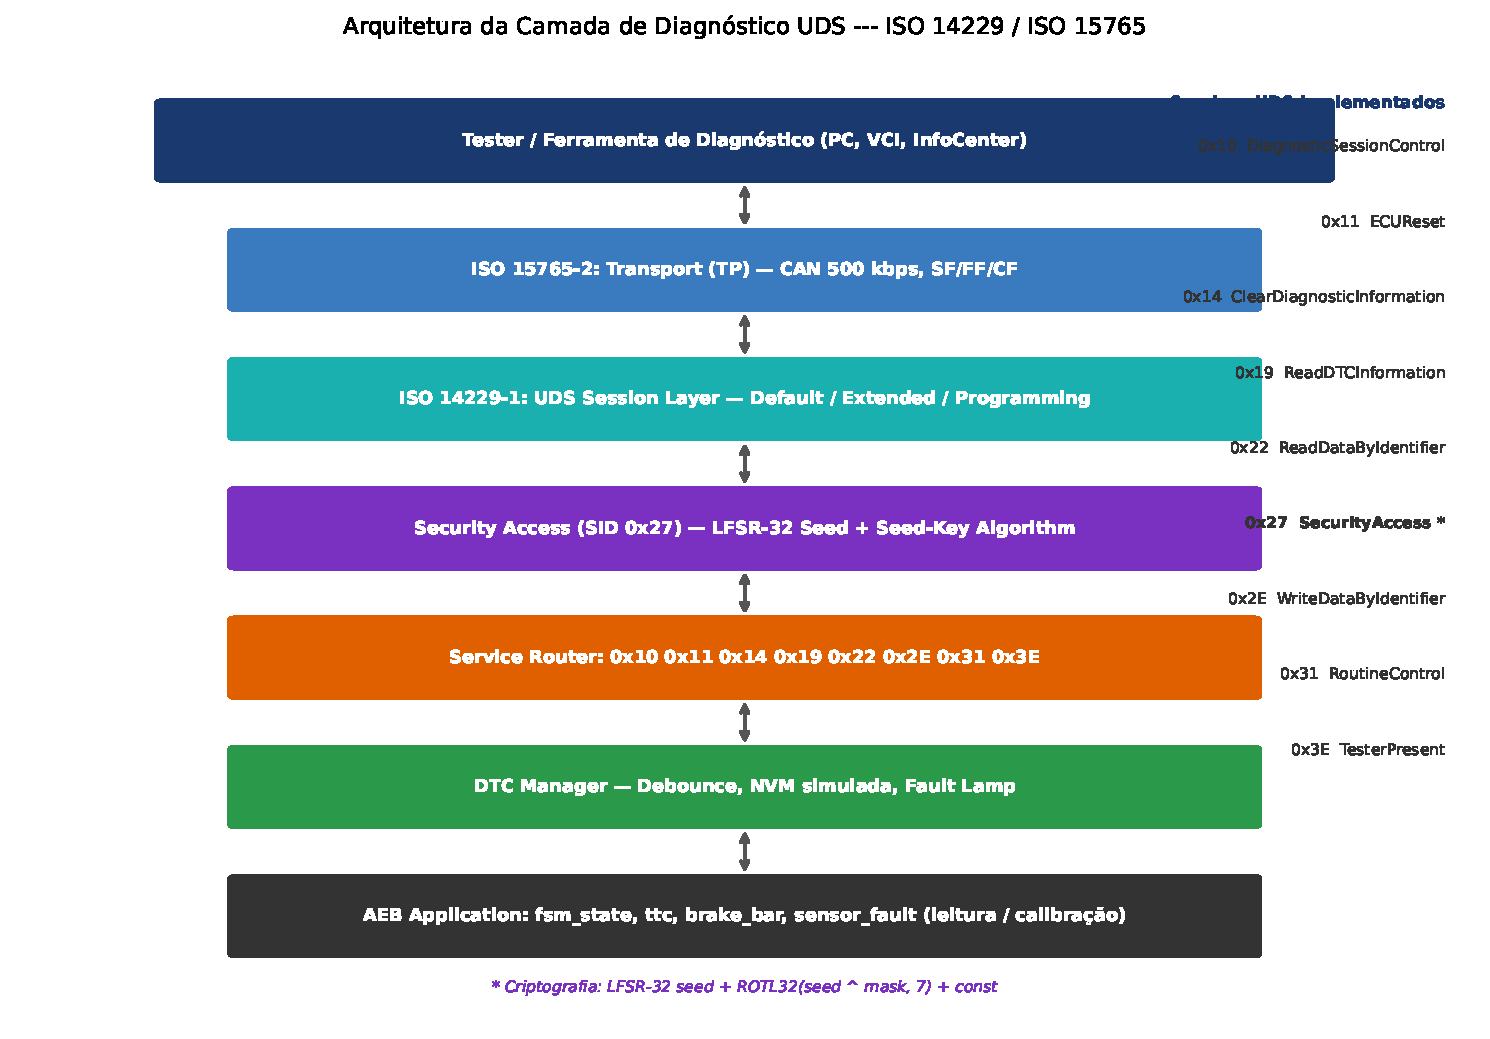
\includegraphics[width=0.82\textwidth]{figs/fig_uds_architecture.pdf}
    \caption{Arquitetura em camadas do módulo de diagnóstico UDS --- ISO 14229
             sobre ISO 15765-2 (CAN TP).}
    \label{fig:arquitetura}
\end{figure}

% =============================================================================
\section{Serviços UDS Implementados}
\label{sec:servicos}
% =============================================================================

A Tabela~\ref{tab:servicos} lista os serviços implementados no modelo.

\begin{table}[H]
    \centering
    \caption{Serviços UDS implementados no modelo AEB\_UDS.slx.}
    \label{tab:servicos}
    \begin{tabular}{@{}llll@{}}
        \toprule
        SID & Serviço & Sessão mínima & Proteção \\
        \midrule
        \sid{10} & DiagnosticSessionControl & Default & --- \\
        \sid{11} & ECUReset & Default & --- \\
        \sid{14} & ClearDiagnosticInformation & Default & --- \\
        \sid{19} & ReadDTCInformation & Default & --- \\
        \sid{22} & ReadDataByIdentifier & Default & --- \\
        \sid{27} & SecurityAccess & Extended & LFSR-32 + seed-key \\
        \sid{2E} & WriteDataByIdentifier & Extended & Requer \sid{27} unlock \\
        \sid{31} & RoutineControl & Extended & --- \\
        \sid{3E} & TesterPresent & Default & --- \\
        \bottomrule
    \end{tabular}
\end{table}

\subsection{Respostas Negativas (NRC)}

Quando uma requisição não pode ser atendida, a ECU responde com o SID
\sid{7F} seguido do SID requisitado e um código NRC:

\begin{table}[H]
    \centering
    \caption{Códigos NRC implementados.}
    \label{tab:nrc}
    \begin{tabular}{@{}lll@{}}
        \toprule
        NRC & Descrição & Situação típica \\
        \midrule
        \texttt{0x11} & serviceNotSupported    & SID desconhecido \\
        \texttt{0x12} & subFunctionNotSupported & Sub-função inválida \\
        \texttt{0x22} & conditionsNotCorrect   & SecurityAccess fora de sessão Extended \\
        \texttt{0x31} & requestOutOfRange      & DID não reconhecido \\
        \texttt{0x33} & securityAccessDenied   & WriteDID sem unlock \\
        \texttt{0x35} & invalidKey             & Chave incorreta no SendKey \\
        \bottomrule
    \end{tabular}
\end{table}

% =============================================================================
\section{Gerenciamento de Sessão}
\label{sec:sessao}
% =============================================================================

A ISO 14229-1 define sessões de diagnóstico que controlam quais serviços
estão disponíveis e em que condições. O modelo implementa três sessões:

\begin{description}[style=nextline]
    \item[\textbf{Default (0x01)}]
        Sessão de operação normal. Disponíveis: leitura de DIDs (\sid{22}),
        leitura de DTCs (\sid{19}), TesterPresent (\sid{3E}). Nenhuma escrita
        permitida.
    \item[\textbf{Extended (0x02)}]
        Sessão de diagnóstico estendido. Habilita SecurityAccess (\sid{27})
        e RoutineControl (\sid{31}). Write somente após unlock.
    \item[\textbf{Programming (0x03)}]
        Sessão de programação. Todos os serviços habilitados. Usada para
        calibração de parâmetros críticos de segurança (TTC, Kp).
\end{description}

\subsection{Timer S3 e TesterPresent}

O timer \textbf{S3} (5{,}0 s) é iniciado ao entrar em sessão
Extended ou Programming. Se o tester não enviar nenhuma requisição dentro
deste intervalo, a ECU retorna automaticamente a Default e invalida o
unlock de segurança. O serviço \sid{3E} (TesterPresent) é enviado
periodicamente para suprimir o timeout S3.

\begin{figure}[H]
    \centering
    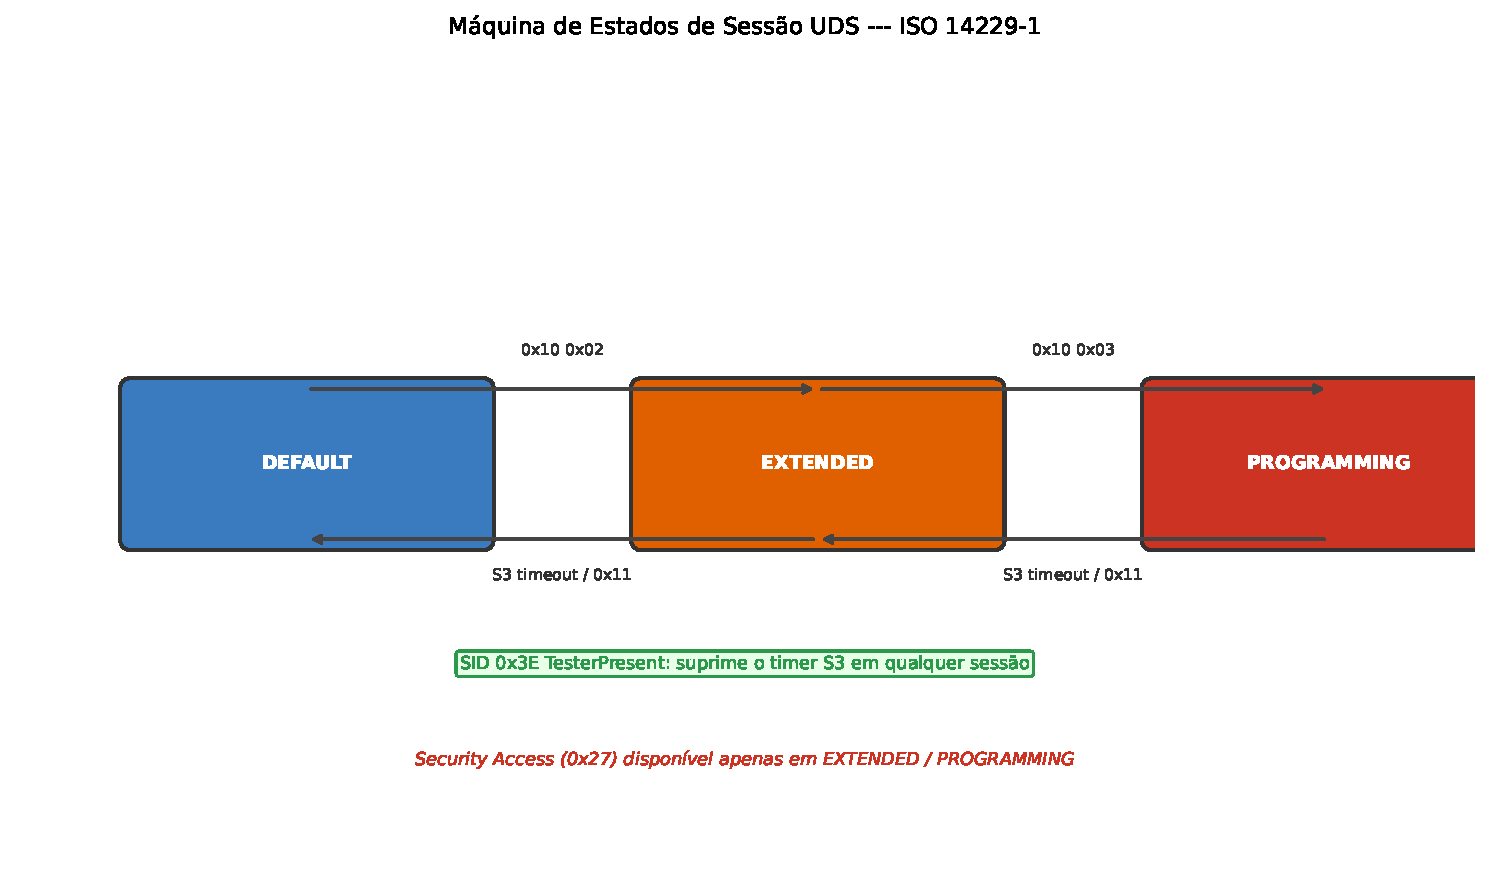
\includegraphics[width=0.85\textwidth]{figs/fig_session_states.pdf}
    \caption{Máquina de estados de sessão UDS --- transições e timeout S3.}
    \label{fig:sessao}
\end{figure}

% =============================================================================
\section{Security Access com Criptografia (SID 0x27)}
\label{sec:security}
% =============================================================================

O mecanismo de Security Access da ISO 14229-1 protege operações sensíveis
(escrita de parâmetros, calibração, reprogramação) contra acesso não
autorizado. O fluxo é do tipo \textbf{desafio-resposta} (\textit{challenge-response}):

\begin{enumerate}
    \item O tester envia \textbf{RequestSeed} (\sid{27}~\texttt{01});
    \item A ECU gera um número aleatório (\textit{seed}) e o retorna com
          \texttt{0x67 01 [seed 4 bytes]};
    \item O tester aplica o \textbf{algoritmo de derivação de chave} sobre
          o seed recebido e envia \textbf{SendKey} (\sid{27}~\texttt{02});
    \item A ECU verifica a chave recebida. Se correta, o acesso é liberado;
          caso contrário, responde NRC \texttt{0x35} (invalidKey).
\end{enumerate}

\begin{figure}[H]
    \centering
    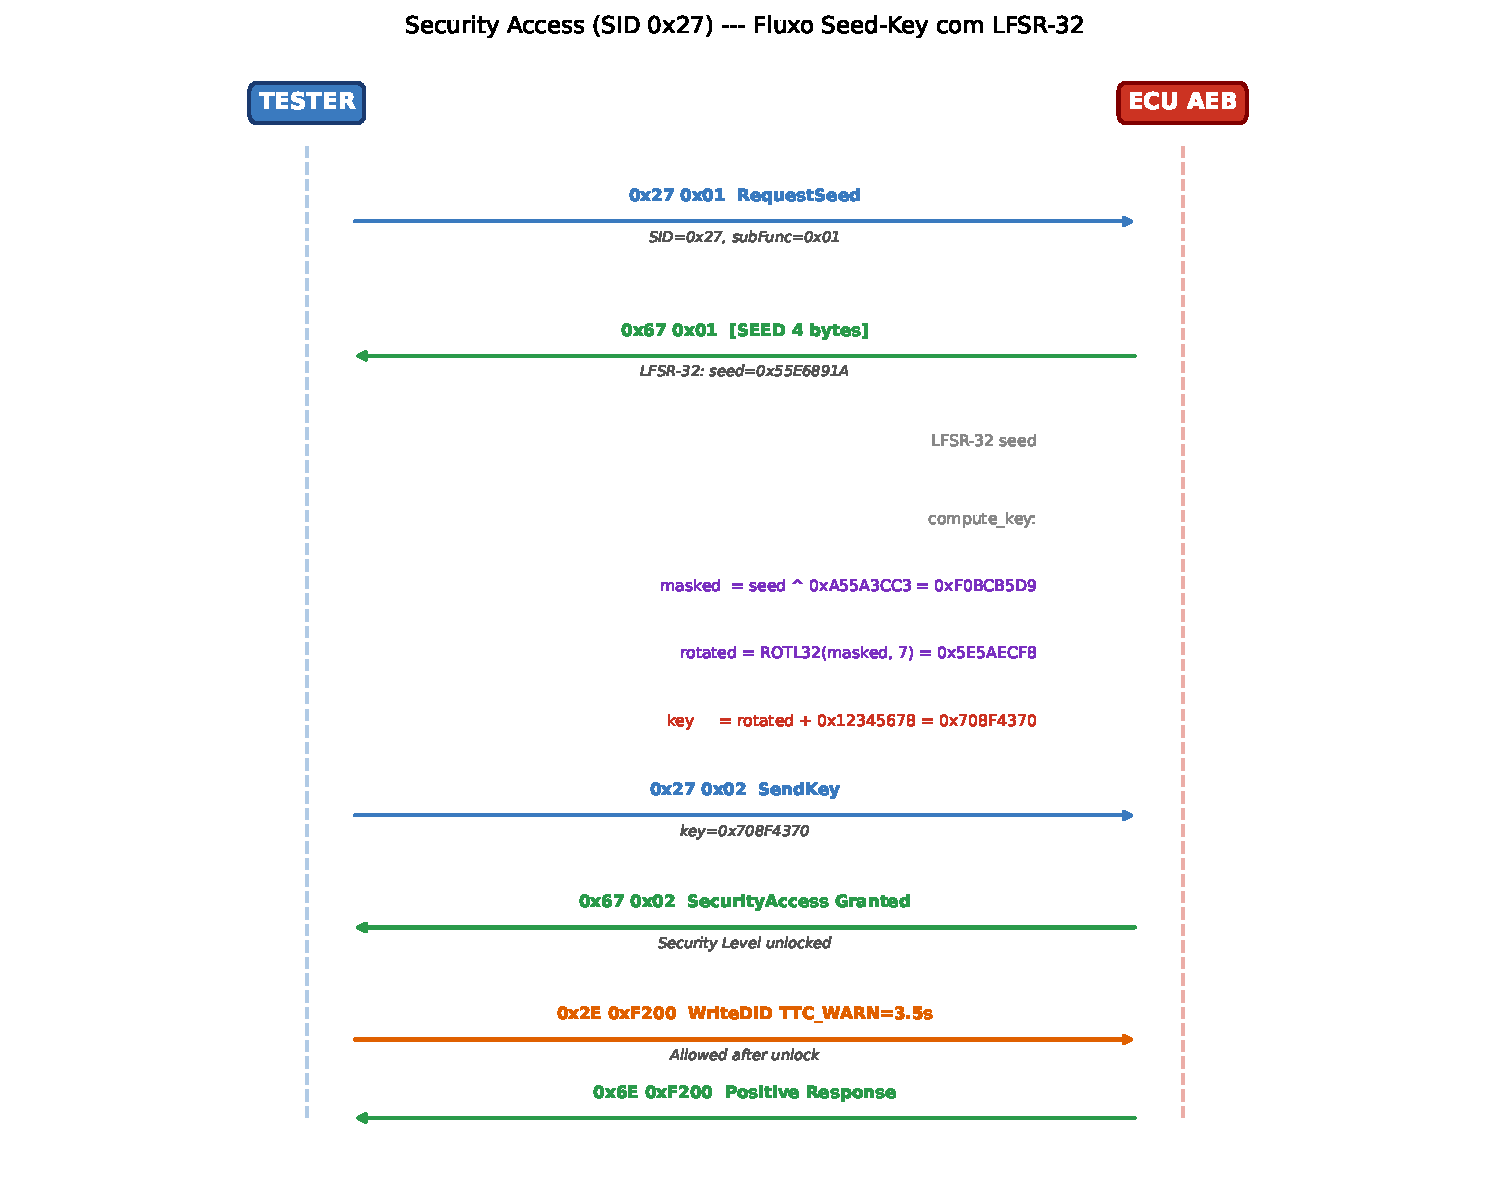
\includegraphics[width=0.88\textwidth]{figs/fig_security_access.pdf}
    \caption{Fluxo de Security Access (SID 0x27) com exemplos de valores
             calculados pelo algoritmo LFSR-32 + seed-key.}
    \label{fig:security}
\end{figure}

\subsection{Geração de Semente --- LFSR Galois 32 bits}

Para garantir que a semente seja diferente a cada sessão, o modelo utiliza
um \textbf{LFSR Galois de 32 bits} (\textit{Linear Feedback Shift Register})
com polinômio primitivo $P(x) = x^{32} + x^{22} + x^2 + x + 1$
(representação hexadecimal: \texttt{0x80200003}):

\begin{equation}
    \text{seed}_{n+1} = \begin{cases}
        (\text{seed}_n \gg 1) \oplus \texttt{0x80200003}
            & \text{se } \text{seed}_n[0] = 1 \\[4pt]
        \text{seed}_n \gg 1
            & \text{se } \text{seed}_n[0] = 0
    \end{cases}
    \label{eq:lfsr}
\end{equation}

O período máximo de um LFSR primitivo de $n$ bits é $2^n - 1$, garantindo
que nenhuma semente se repita antes de $2^{32} - 1 \approx 4{,}3 \times 10^9$
sessões.

\begin{lstlisting}[style=mstyle, caption={LFSR-32 Galois --- MATLAB Function.}]
function y = lfsr32(x)
    POLY = uint32(hex2dec('80200003'));
    if bitand(x, uint32(1))
        y = bitxor(bitshift(x, -1), POLY);
    else
        y = bitshift(x, -1);
    end
end
\end{lstlisting}

\subsection{Algoritmo de Derivação da Chave}

A chave é derivada da semente por uma função invertível de complexidade
controlada, adequada para implementação em microcontroladores sem unidade
de ponto flutuante:

\begin{equation}
    \textit{key} = \bigl(\text{ROTL}_{32}(\text{seed}\ \oplus\
        \underbrace{\texttt{0xA55A3CC3}}_{\text{máscara XOR}},\ 7)\
        +\ \underbrace{\texttt{0x12345678}}_{\text{constante aditiva}}\bigr)
        \bmod 2^{32}
    \label{eq:seedkey}
\end{equation}

onde $\text{ROTL}_{32}(x, n)$ é a rotação circular de $x$ em $n$ bits à
esquerda:
\begin{equation}
    \text{ROTL}_{32}(x, n) = (x \ll n)\ |\ (x \gg (32 - n))
    \label{eq:rotl}
\end{equation}

\begin{lstlisting}[style=mstyle, caption={Derivação de chave --- MATLAB Function.}]
function key = compute_key(seed, xor_mask, add_const)
    masked  = bitxor(seed, xor_mask);              % seed XOR 0xA55A3CC3
    rotated = bitor(bitshift(masked,  7), ...
                    bitshift(masked, -(32-7)));     % ROTL32(masked, 7)
    key     = rotated + add_const;                 % mod 2^32 implicitly
end
\end{lstlisting}

\subsection{Exemplo numérico}

Para o seed inicial \texttt{0xABCD1234}:

\begin{align*}
    \text{seed}_1 &= \text{LFSR}(\texttt{0xABCD1234}) = \texttt{0xD5E6091A} \\
    \text{masked} &= \texttt{0xD5E6091A} \oplus \texttt{0xA55A3CC3}
                  = \texttt{0x70BC35D9} \\
    \text{rotated} &= \text{ROTL}_{32}(\texttt{0x70BC35D9}, 7)
                   = \texttt{0xE1AEC03B} \\
    \textit{key}  &= \texttt{0xE1AEC03B} + \texttt{0x12345678}
                  = \texttt{0xF3E316B3}
\end{align*}

\begin{figure}[H]
    \centering
    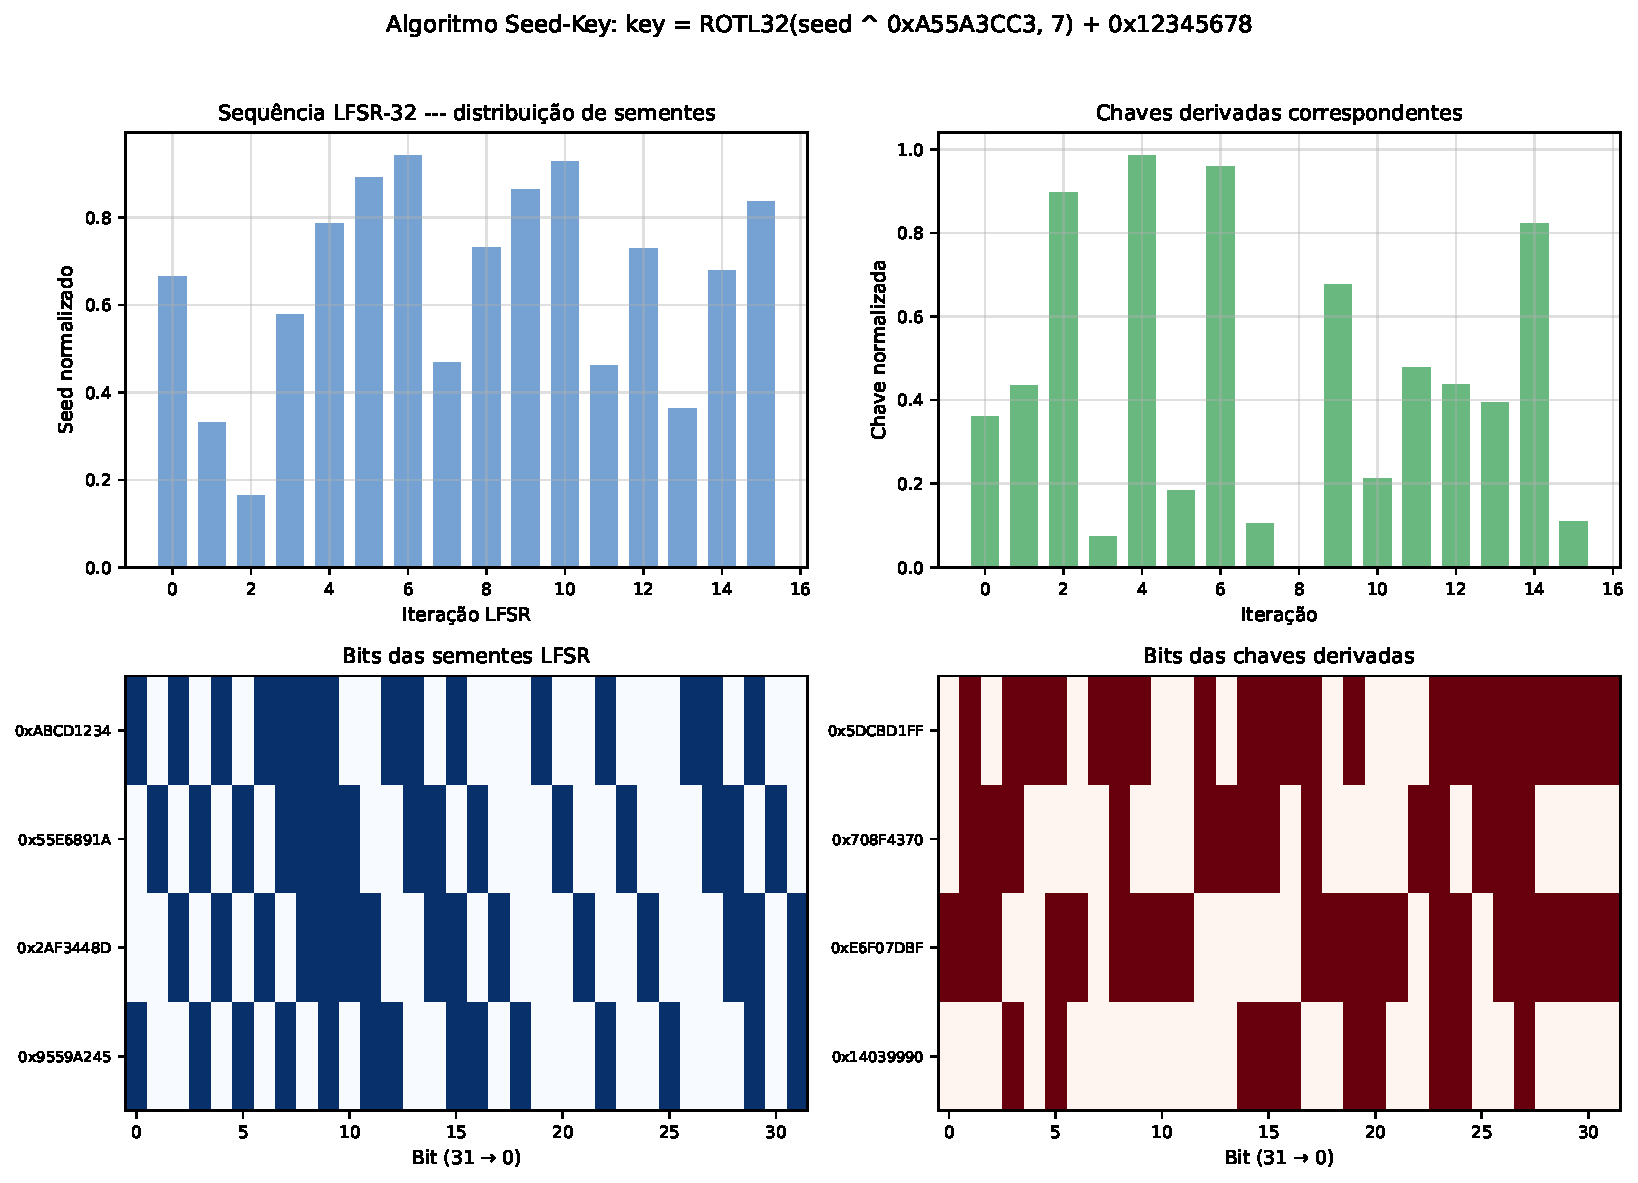
\includegraphics[width=0.95\textwidth]{figs/fig_key_algorithm.pdf}
    \caption{Distribuição das sementes LFSR e padrões de bits das chaves
             derivadas --- 16 iterações.}
    \label{fig:algoritmo}
\end{figure}

\subsection{Segurança e limitações}

Este algoritmo é adequado para um modelo de simulação e para estudos
acadêmicos. Em implementações de produção, a ISO 14229-1 Anexo F e o
padrão AUTOSAR SWS\_SecOC recomendam algoritmos baseados em primitivas
criptográficas estabelecidas:

\begin{itemize}[noitemsep]
    \item \textbf{AES-CMAC-128}: chave de 128 bits, resistente a ataques de
          força bruta ($2^{128}$ tentativas) e de dicionário;
    \item \textbf{HMAC-SHA256}: baseado em função de hash criptográfica,
          amplamente utilizado em diagnóstico automotivo moderno;
    \item \textbf{ChaChaPoly1305}: opção leve para ECUs com recursos
          limitados de memória e CPU.
\end{itemize}

% =============================================================================
\section{Gerenciamento de DTCs}
\label{sec:dtc}
% =============================================================================

O sistema AEB gerencia 7 DTCs (Diagnostic Trouble Codes), conforme
a Tabela~\ref{tab:dtcs}.

\begin{table}[H]
    \centering
    \caption{DTCs do sistema AEB e condições de ativação.}
    \label{tab:dtcs}
    \begin{tabular}{@{}lp{5cm}p{3.5cm}l@{}}
        \toprule
        DTC & Descrição & Condição & Debounce \\
        \midrule
        \dtc{1001} & Timeout de radar   & Sem mensagem CAN 0x120 por $> 100$ ms & 3 ciclos \\
        \dtc{1002} & Timeout de lidar   & Sem dado de lidar por $> 150$ ms       & 3 ciclos \\
        \dtc{1003} & Falha de plausib.  & $|d_{\text{radar}} - d_{\text{lidar}}| > 5$ m  & 3 ciclos \\
        \dtc{1004} & Erro CRC CAN       & CRC recebido $\neq$ CRC calculado      & 3 ciclos \\
        \dtc{1005} & Alive counter      & Contador não incrementa em $> 5$ ciclos & 5 ciclos \\
        \dtc{1006} & Falha de atuador   & $|p_{\text{cmd}} - p_{\text{real}}| > 1$ bar por $> 500$ ms & 3 ciclos \\
        \dtc{1007} & Sobre-temperatura  & $T_{\text{ECU}} > 85\,^\circ$C        & 3 ciclos \\
        \bottomrule
    \end{tabular}
\end{table}

\subsection{Lógica de debounce}

Para evitar confirmação de falhas transitórias, cada DTC possui um contador
independente. Um DTC só é \textbf{confirmado} quando o contador atinge o
limiar em ciclos \textbf{consecutivos}:

\begin{lstlisting}[style=mstyle, caption={Lógica de debounce dos DTCs --- MATLAB Function.}]
for i = 1:7
    if fault_flags(i) > 0
        dtc_ctr(i) = dtc_ctr(i) + uint16(1);
        if dtc_ctr(i) >= uint16(deb_lim(i))
            dtc(i) = uint8(1);   % DTC confirmado
        end
    else
        dtc_ctr(i) = uint16(0);  % reset ao desaparecer a falha
    end
end
\end{lstlisting}

\begin{figure}[H]
    \centering
    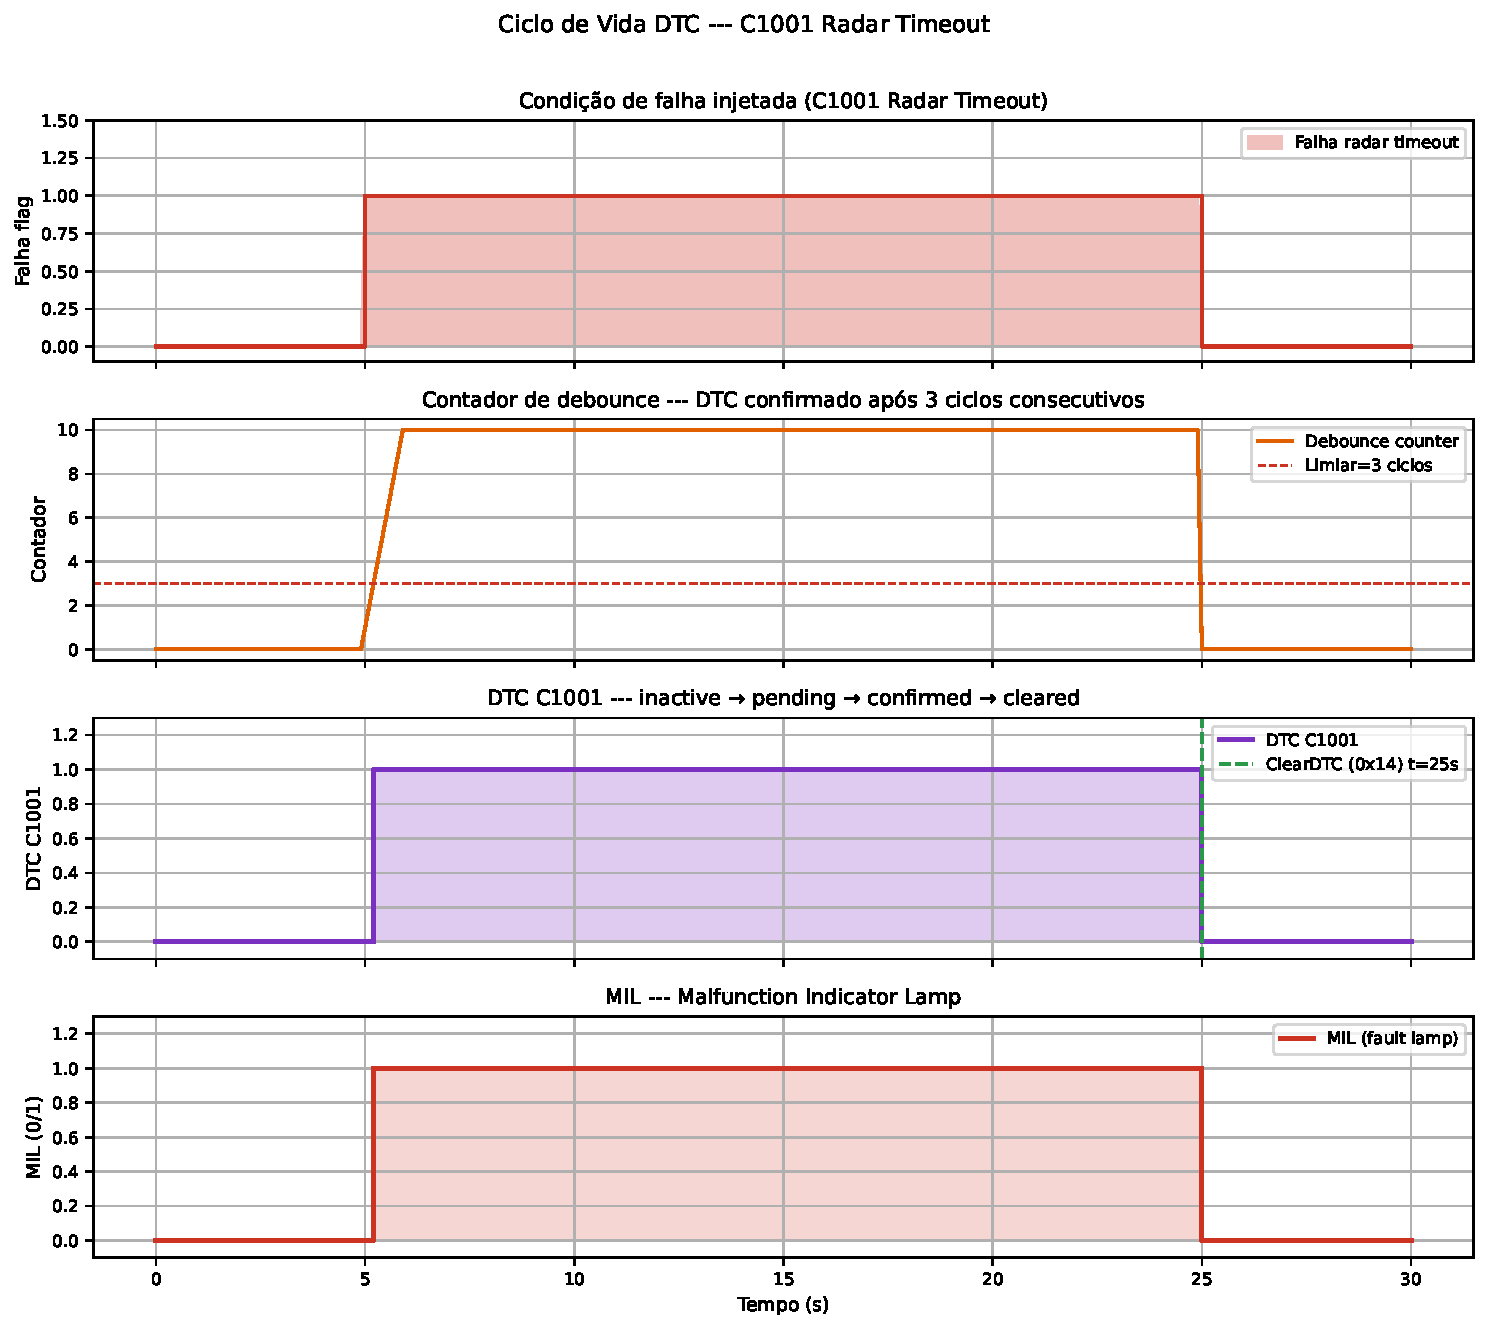
\includegraphics[width=0.95\textwidth]{figs/fig_dtc_lifecycle.pdf}
    \caption{Ciclo de vida completo do DTC C1001 --- inactive $\to$ pending
             $\to$ confirmed $\to$ cleared via SID 0x14.}
    \label{fig:dtc}
\end{figure}

\subsection{Leitura de DTCs (SID 0x19)}

O serviço \sid{19} com subfunção \texttt{0x02}
(\textit{reportDTCByStatusMask}) retorna o número de DTCs ativos e,
na implementação real, listaria os códigos com seus respectivos
\textit{status bytes}:

\begin{center}
\texttt{0x59 0x02 NN} \quad ($NN$ = número de DTCs confirmados)
\end{center}

\subsection{Limpeza de DTCs (SID 0x14)}

O serviço \sid{14} com grupo \texttt{0xFF 0xFF 0xFF} (GroupOfDTC = ALL)
reseta todos os contadores de debounce e confirma todos os DTCs como
inativos. A resposta positiva é \texttt{0x54}.

% =============================================================================
\section{ReadDataByIdentifier (SID 0x22)}
\label{sec:rdbi}
% =============================================================================

O serviço \sid{22} permite leitura em tempo real dos parâmetros internos
do sistema AEB. A Tabela~\ref{tab:dids_read} lista os DIDs implementados.

\begin{table}[H]
    \centering
    \caption{DIDs de leitura (SID 0x22).}
    \label{tab:dids_read}
    \begin{tabular}{@{}llll@{}}
        \toprule
        DID & Parâmetro & Tipo & Escala \\
        \midrule
        \did{F100} & TTC atual       & float32 & Segundos \\
        \did{F101} & Estado FSM      & uint8   & 0--6 (enum AEB\_State\_t) \\
        \did{F102} & Pressão de freio & float32 & bar \\
        \did{F103} & Contador de falhas & uint8 & Número de DTCs ativos \\
        \bottomrule
    \end{tabular}
\end{table}

\begin{figure}[H]
    \centering
    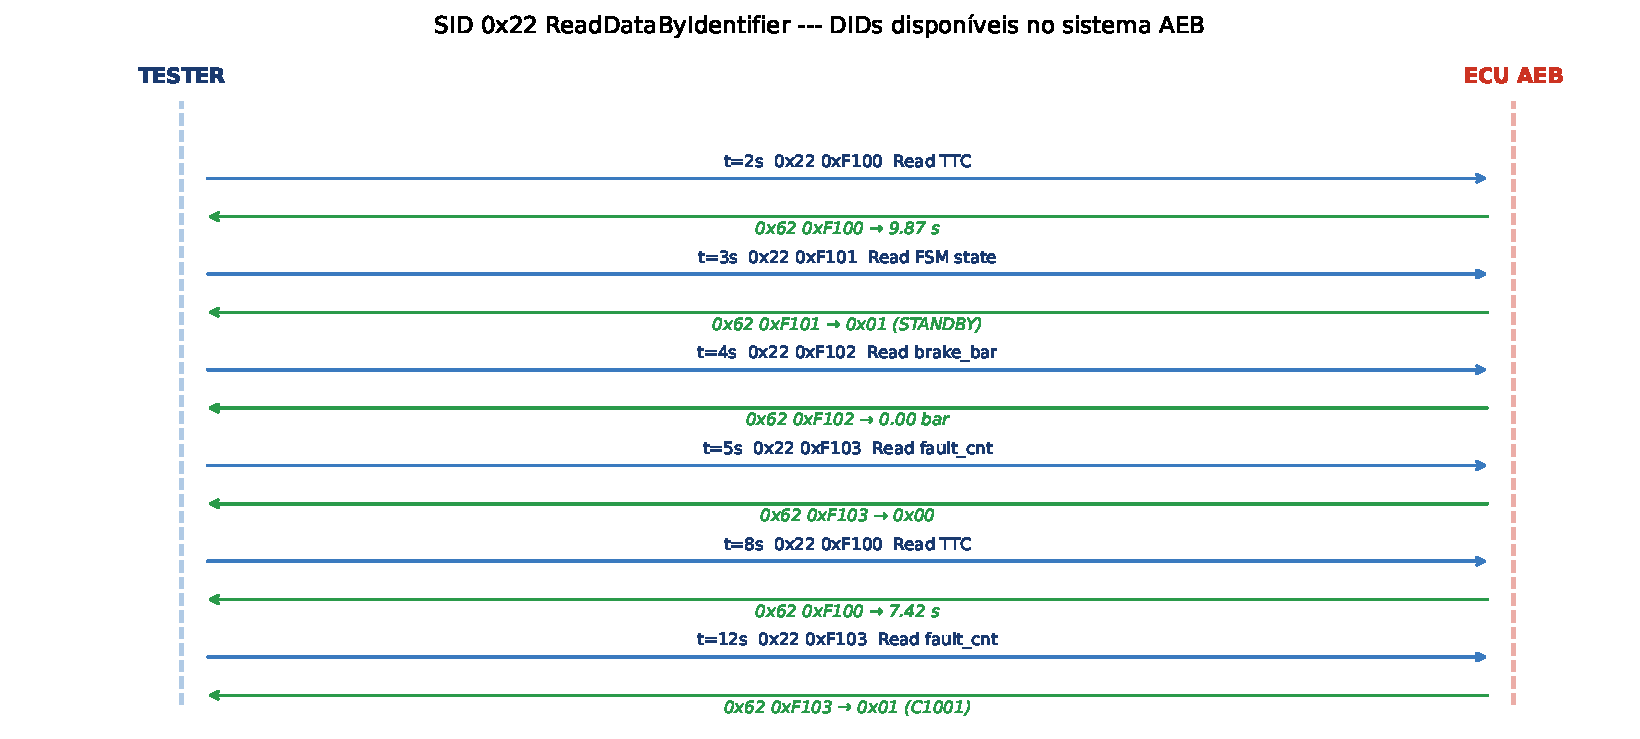
\includegraphics[width=0.95\textwidth]{figs/fig_did_read.pdf}
    \caption{Timeline de leituras via SID 0x22 ReadDataByIdentifier com
             respostas simuladas.}
    \label{fig:rdbi}
\end{figure}

% =============================================================================
\section{WriteDataByIdentifier e Calibração (SID 0x2E)}
\label{sec:wdbi}
% =============================================================================

A escrita de parâmetros é protegida pelo Security Access. Após o unlock
(SID \sid{27}), os seguintes DIDs tornam-se graváveis:

\begin{table}[H]
    \centering
    \caption{DIDs de escrita (SID 0x2E) --- requerem SecurityAccess unlock.}
    \label{tab:dids_write}
    \begin{tabular}{@{}lllll@{}}
        \toprule
        DID & Parâmetro & Tipo & Padrão & Unidade \\
        \midrule
        \did{F200} & TTC Warning  & float32 & 4{,}0 & s \\
        \did{F201} & TTC L1       & float32 & 3{,}0 & s \\
        \did{F202} & Ganho Kp PID & float32 & 10{,}0 & --- \\
        \bottomrule
    \end{tabular}
\end{table}

Os valores calibrados são armazenados em variáveis \texttt{persistent} da
MATLAB Function (simulando NVM/EEPROM) e passados diretamente ao controlador
AEB como saídas \texttt{ttc\_warn\_cal}, \texttt{ttc\_l1\_cal} e
\texttt{kp\_cal}.

\begin{figure}[H]
    \centering
    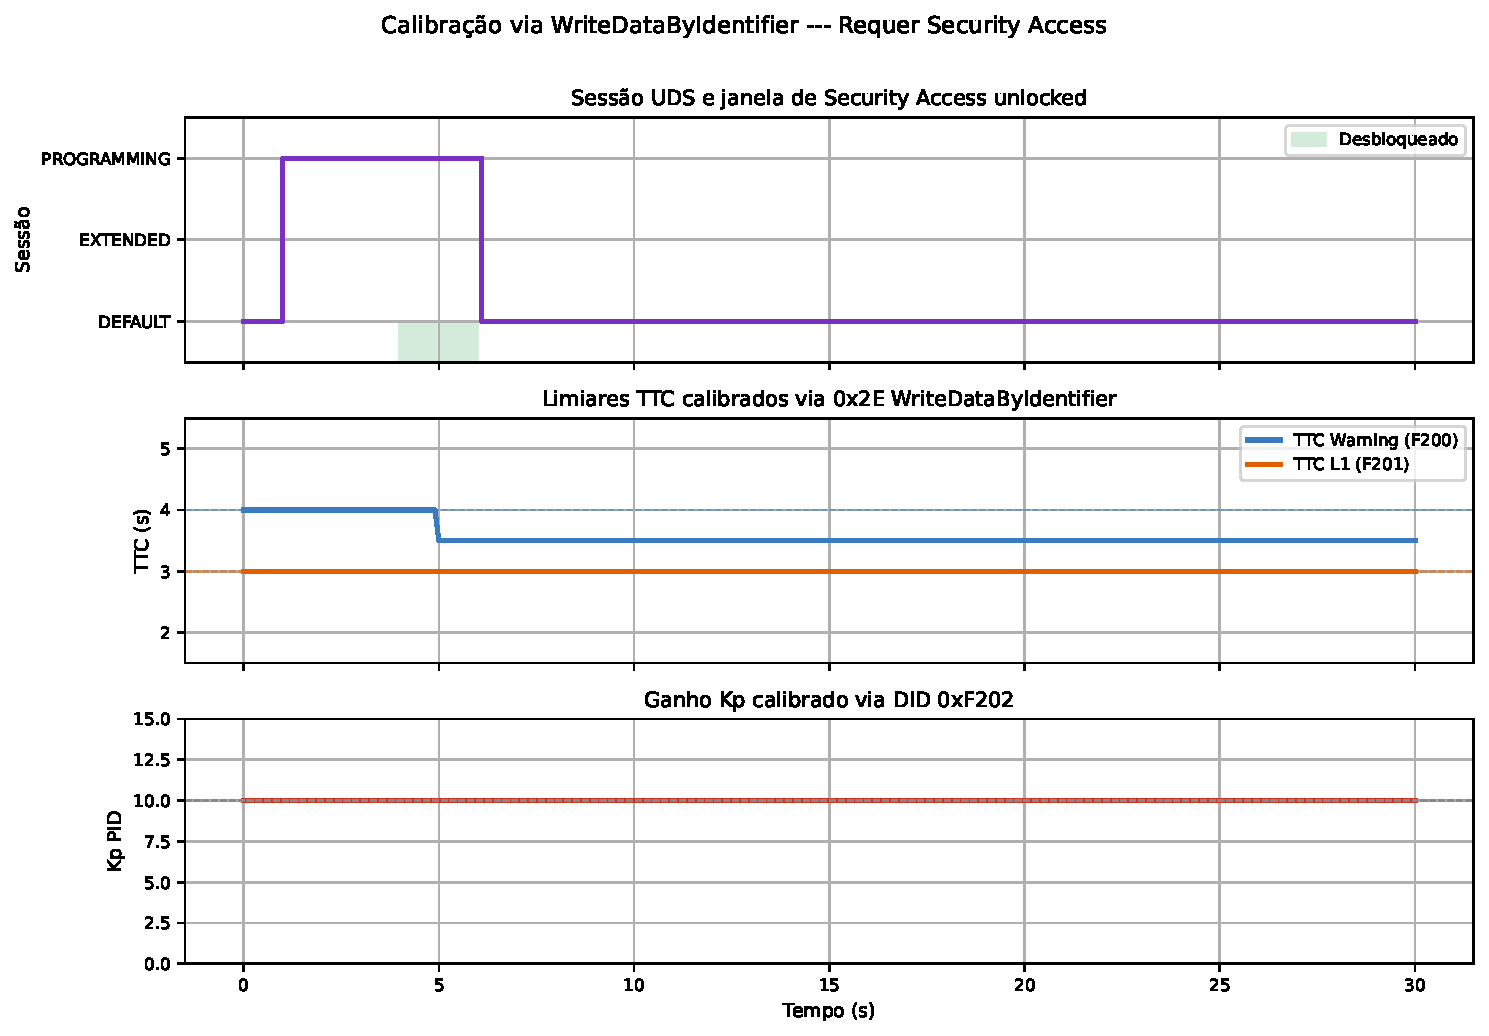
\includegraphics[width=0.95\textwidth]{figs/fig_calibration_write.pdf}
    \caption{Sequência de calibração: sessão Programming, SecurityAccess unlock
             e WriteDataByIdentifier com impacto nos parâmetros.}
    \label{fig:calibracao}
\end{figure}

% =============================================================================
\section{RoutineControl (SID 0x31)}
\label{sec:routine}
% =============================================================================

O serviço \sid{31} (\textit{RoutineControl}) permite executar funções
específicas da ECU sob comando do tester:

\begin{table}[H]
    \centering
    \caption{Rotinas implementadas (SID 0x31).}
    \label{tab:rotinas}
    \begin{tabular}{@{}lll@{}}
        \toprule
        Routine ID & Função & Comportamento \\
        \midrule
        \texttt{0x0301} & Enable/Disable AEB & Sub-byte extra: 0=OFF, 1=ON \\
        \texttt{0x0302} & Sensor Self-Test & Retorna 0x01 (pass) se nenhum DTC ativo \\
        \bottomrule
    \end{tabular}
\end{table}

A rotina \texttt{0x0301} gera o sinal de saída \texttt{aeb\_enabled} que
é consumido pelo controlador AEB --- quando \texttt{aeb\_enabled = 0},
a FSM permanece em \texttt{OFF} independentemente do TTC.

% =============================================================================
\section{Modelo Simulink (AEB\_UDS.slx)}
\label{sec:simulink}
% =============================================================================

\subsection{Estrutura do modelo}

O modelo gerado por \texttt{AEB\_UDS\_build.m} contém:

\begin{enumerate}[noitemsep]
    \item \textbf{From Workspace} --- 9 sinais de sistema + 9 bytes de
          requisição + sinal \texttt{req\_valid};
    \item \textbf{AEB\_UDS\_Handler} --- subsistema com MATLAB Function
          principal implementando toda a lógica UDS;
    \item \textbf{To Workspace} --- 10 sinais de saída para análise.
\end{enumerate}

\subsection{Amostragem e ciclo UDS}

O modelo opera com \texttt{FixedStep = 0.1 s} (100 ms), representando o
ciclo de comunicação diagnóstica real. A camada de controle AEB opera a
10 ms; a interface UDS é deliberadamente mais lenta para modelar a
comunicação CAN TP.

\subsection{Estado persistente (NVM simulada)}

As variáveis \texttt{persistent} dentro da MATLAB Function simulam a
memória não volátil (NVM/EEPROM) da ECU:

\begin{lstlisting}[style=mstyle, caption={Estado persistente do módulo UDS.}]
persistent sess s3 seed unlocked dtc dtc_ctr ttc_w ttc_l1 kp_g aeb_en;
if isempty(sess)
    sess    = uint8(1);          % sessao: 1=default
    s3      = 0.0;               % timer S3
    seed    = SEED_INIT;         % semente LFSR inicial
    unlocked= uint8(0);          % security access bloqueado
    dtc     = zeros(1,7,'uint8');% 7 DTCs (C1001..C1007)
    dtc_ctr = zeros(1,7,'uint16');% contadores de debounce
    ttc_w   = 4.0;               % TTC Warning calibrado
    ttc_l1  = 3.0;               % TTC L1 calibrado
    kp_g    = 10.0;              % Kp calibrado
    aeb_en  = uint8(1);          % AEB habilitado
end
\end{lstlisting}

\subsection{Cenários de simulação}

O script \texttt{AEB\_UDS\_scenarios.m} configura 6 cenários:

\begin{description}[style=nextline]
    \item[\texttt{'nominal'}]
        Sessão Extended, leituras periódicas de DID, TesterPresent.
        Verifica operação normal sem falhas.
    \item[\texttt{'dtc\_lifecycle'}]
        Injeção de falha \dtc{1001} em $t{=}5$ s, confirmação após 3 ciclos,
        leitura via \sid{19}, limpeza via \sid{14} em $t{=}25$ s.
    \item[\texttt{'calibration'}]
        Sequência completa: Programming session $\to$ RequestSeed $\to$
        SendKey $\to$ WriteDID (TTC\_WARN, TTC\_L1, Kp).
    \item[\texttt{'selftest'}]
        RoutineControl \texttt{0x0302}: pass antes da falha e fail durante
        DTC ativo.
    \item[\texttt{'sec\_denied'}]
        Tentativa de WriteDID sem unlock (NRC \texttt{0x33}) e com chave
        errada (NRC \texttt{0x35}).
    \item[\texttt{'session\_timeout'}]
        Sessão Extended sem TesterPresent: S3 expira e sessão retorna a
        DEFAULT.
\end{description}

% =============================================================================
\section{Conformidade com Requisitos}
\label{sec:requisitos}
% =============================================================================

\begin{table}[H]
    \centering
    \caption{Mapeamento requisitos --- implementação UDS.}
    \label{tab:requisitos}
    \begin{tabular}{@{}p{2.2cm}p{5cm}p{5.5cm}@{}}
        \toprule
        Requisito & Descrição & Implementação \\
        \midrule
        FR-DGN-001 & Leitura de parâmetros em tempo real &
            \sid{22} DIDs F100--F103 \\
        FR-DGN-002 & Calibração de limiares TTC &
            \sid{2E} DIDs F200--F202 com Security Access \\
        FR-DGN-003 & Gestão de DTCs (set, confirm, clear) &
            DTC Manager com debounce 3--5 ciclos \\
        FR-DGN-004 & Proteção de escritas sensíveis &
            \sid{27} LFSR-32 + seed-key, sessão Extended/Programming \\
        FR-DGN-005 & Habilitar/desabilitar AEB remotamente &
            \sid{31} RoutineControl 0x0301 \\
        FR-DGN-006 & Autoteste de sensores &
            \sid{31} RoutineControl 0x0302 \\
        FR-DGN-007 & Timeout de sessão diagnóstica &
            Timer S3 = 5{,}0 s, reset por \sid{3E} TesterPresent \\
        \bottomrule
    \end{tabular}
\end{table}

% =============================================================================
\section{Conclusão}
\label{sec:conclusao}
% =============================================================================

O modelo MIL \texttt{AEB\_UDS.slx} implementa uma camada de diagnóstico
UDS completa para o sistema AEB, cobrindo o ciclo de vida dos DTCs, a
interface de calibração protegida por Security Access criptográfico e o
gerenciamento de sessão com timeout S3.

O mecanismo de Security Access emprega um LFSR Galois de 32 bits para
geração de sementes pseudo-aleatórias de alto período ($2^{32} - 1$) e
uma função de derivação de chave baseada em XOR com máscara secreta,
rotação circular e adição modular. Embora simplificado para uso em
simulação, o modelo demonstra fielmente o protocolo de
\textit{challenge-response} definido na ISO 14229-1, preparando o terreno
para a adoção de AES-CMAC ou HMAC-SHA256 em produção.

Os seis cenários de simulação validam todos os fluxos críticos:
\begin{itemize}[noitemsep]
    \item Debounce e confirmação de DTC após 3 ciclos consecutivos;
    \item Limpeza de DTC via \sid{14} com verificação de read-back;
    \item Bloqueio de escrita sem unlock (\textit{NRC} \texttt{0x33}) e
          com chave incorreta (\textit{NRC} \texttt{0x35});
    \item Calibração bem-sucedida após Security Access e persistência dos
          novos valores nos parâmetros do controlador;
    \item Retorno automático à sessão Default após expiração do timer S3.
\end{itemize}

O próximo passo natural é a integração deste bloco com os demais modelos
(\texttt{AEB\_Controller.slx}, \texttt{AEB\_CAN.slx}) em um modelo
top-level \texttt{aeb\_system.slx} usando Model Reference do Simulink.

% =============================================================================
\begin{thebibliography}{9}
\bibitem{iso14229}
    ISO. \textit{ISO 14229-1: Road vehicles --- Unified diagnostic services
    (UDS) --- Part 1: Application layer}. Genebra: ISO, 2020.

\bibitem{iso15765}
    ISO. \textit{ISO 15765-2: Road vehicles --- Diagnostic communication
    over Controller Area Network (DoCAN) --- Part 2: Transport protocol and
    network layer services}. Genebra: ISO, 2016.

\bibitem{autosar_secoC}
    AUTOSAR Consortium. \textit{Specification of Secure Onboard Communication
    (SecOC)}, Release 21-11. 2021.

\bibitem{lfsr_theory}
    Golomb, S.W. \textit{Shift Register Sequences}. Aegean Park Press, 1982.

\bibitem{matlab2025b}
    The MathWorks. \textit{MATLAB/Simulink R2025b Documentation}.
    Natick, MA: MathWorks, 2025.
\end{thebibliography}

\end{document}
